\documentclass[12pt,a4paper]{article}

\usepackage{alltt}
\usepackage[utf8]{inputenc}
\usepackage[english]{babel}
\usepackage{amsmath}
\usepackage{amsfonts}
\usepackage{amssymb}
\usepackage{indentfirst}
\usepackage{setspace}
\usepackage[pdftex]{graphicx}
\usepackage{caption}
\usepackage{subcaption}
\usepackage{textcomp}
\usepackage{array}
\usepackage{listings}
\usepackage{color}
\usepackage{tikz} % для создания иллюстраций
\usepackage{hyperref}

\newcommand{\infers}{\,\to\,}
\newcommand{\tinfers}{\;\Rightarrow\;}

%\voffset = -118pt
%\textheight = 820pt
%\hoffset = -100pt
%\textwidth = 550pt
\newcommand{\htext}{0.46\textwidth}
\newcommand{\hstext}{0.45\textwidth}

\newcommand{\mat}[1]{\overline{#1}}
\newcommand{\framed}[1]{\tikz[baseline=(char.base)]{\node[shape=rectangle,draw,inner sep=4pt] (char) {#1};}}

%opening
\title{}
\author{}

\begin{document}


% TEAM.
\parbox{0.333\textwidth}{
	Maksim Velikanov \\[0mm]
}
% In der Mitte der Name der Veranstaltung.
\parbox{0.333\textwidth}{\vspace*{1mm}\begin{center}\large\bf%
		HPC with C++\\[0mm]
		SS 24\\[0mm]
\end{center}}
\parbox{0.333\textwidth}{
	\begin{flushright}
		Project report\\[0mm]
		13.09.2024\\[0mm]
	\end{flushright}
}
\par\vspace{-5mm}
\definecolor{freiburg-gray}{rgb}{0.68,0.68,0.68}
\vspace*{2mm}
\raisebox{1.19cm}{%
	\textcolor{freiburg-gray}{\rule{\textwidth}{1.1mm}}}

\bigskip




\section{Introduction}

I completed the milestones until no. 6. The implemented program is capable of generating a cubic lattice or using a precomputed one; running the simulation under control without the cluster vaporizing; monitoring the energies; saving the cluster for visualization.

The theoretical base is present in \hyperref[methods]{methods}, the overview of implementation and results in \hyperref[implementation]{implementation}, and \hyperref[conclusion]{conclusion} at the end.

\section{Methods}
\label{methods}

The key components of Molecular Dynamics are following:

\begin{enumerate}
	\item Update atom position and velocity, given constant force for a small time step --- {\bf Velocity-Verlet integrator}
	\item Estimate force between particles from the potential energy --- {\bf Lennard-Jones potential and Embedded Atom method potential}
	\item Prevent explosion of the system by connecting it to a constant-temperature heat bath --- {\bf Berendsen Thermostat}
\end{enumerate}

\newpage
\subsection*{Velocity-Verlet integrator}

The movement is approximated by assuming constant force and making small time steps. We take Newton's law and definition of velocity, using Taylor formula, we get the approximation equations. Was rediscovered by Loup Verlet \cite{verlet} for Molecular Dynamics simulation.

\[ \dot{\mat{v}}_i(t) = \cfrac{\mat{f}_i(t)}{m_i} \]
\[ \dot{\mat{r}}_i(t) = \mat{v}_i(t) \]

Integration, predictor step:
\[
v_i(t + \Delta t/2) = v_i(t) + \cfrac{1}{2m_i} f_i(t) \Delta t
\]
\[ r_i(t+\Delta t) = r_i(t) + v_i(t+ \Delta t/2) \Delta t \]

Corrector step:
\[ v_i(t+\Delta t) = v_i(t+\Delta t/2) + \cfrac{1}{2m_i}f_i(t+\Delta t) \Delta t \]

{\bf Implementation} --- src/atoms.h, src/verlet.cpp, src/verlet.h, tests/test\_verlet.cpp

\subsection*{Lennard Jones potential}

Here we derive a formula to compute the force from potential energy. By definition of pair potential:
\[
E_{pot} = \sum_{i<j} V(r_{ij})
\]

Lennard-Jones potential \cite{lennard-jones} is sum of Pauli Repulsion (repulsive force) and London Dispersion (attractive force). These interactions act even on uncharged atoms.

\[
V_{ij}(r) = 4\epsilon \left( \Bigl(\cfrac{\sigma}{r}\Bigr)^{12} - \Bigl(\cfrac{\sigma}{r}\Bigr)^{6} \right)
\]

By definition of energy, force is the derivative of energy by position.
\[
\mat{f}_k = \left( \begin{aligned}
	& - \partial E / \partial x_k \\
	& - \partial E / \partial y_k \\
	& - \partial E / \partial z_k \\
\end{aligned} \right) = \sum_i \cfrac{\partial V}{\partial r_{ik}} {\hat r_{ik}} \text{\ (unit vector)}
\]

Let's compute for one of the dimensions.
\[
\cfrac{\partial V_{ij}}{\partial x_k} = \text{(chain rule by vector length)} \cfrac{\partial V_{ij}}{\partial r_{ij}} \cfrac{\partial r_{ij}}{\partial x_k}
\]

\[ \cfrac{\partial r_{ij}}{\partial x_k} = \cfrac{\partial \sqrt{(x_j-x_i)^2 + \ldots}}{\partial x_k} = (*) \]
Remember: \( (\sqrt{u})' = \cfrac{1}{2\sqrt{u}} u' \)

\[
(*) = \cfrac{1}{2r_{ij}} \cfrac{(x_j-x_i)^2+\ldots}{\partial x_k} = \cfrac{1}{r_{ij}} \cdot (x_j-x_i) \cdot \Bigl(\cfrac{\partial x_j}{\partial x_k} - \cfrac{\partial x_i}{\partial x_k}\Bigr)
\]
Here is a pair of atoms $i$ and $j$. We want the force for atom $k$. If \(k\neq i\) and \(k\neq j\), the expression is 0.

\[
(*) = \left( \begin{aligned}
	& (x_j - x_i) (\delta_{jk} - \delta_{ik}) / r_{ij} \\
	& (y_j - y_i) (\delta_{ik} - \delta_{jk}) / r_{ij} \\
	& (z_j - z_i) (\delta_{ik} - \delta_{jk}) / r_{ij} \\
\end{aligned} \right) 
\]

\[
k=j \infers (x_k-x_i)(1-0)/r_{ik},\ (*) = {\hat r_{ik}}
\]
\[
k=i \infers (x_j-x_k)(0-1)/r_{kj},\ (*) = {\hat r_{jk}}
\]

When we take the derivative of energy, only the pairs, where one of the atoms is \(k\), are left. The derivative is exactly the same for \(V_{ij}\) and \(V_{ji}\).

{\centering\framed{ \( \mat{f}_k = - \sum_i \cfrac{\partial V}{\partial r} {\hat r_{ik}} \) }\\}

Last piece in the puzzle is derivative of potential by distance.

\[
\cfrac{\partial V}{\partial r} = 4\epsilon (\sigma^{12} (-12) r^{-13} - \sigma^6\cdot 6\cdot r^{-7})
\]

\subsection*{Berendsen thermostat}

As the molecular dynamics system evolves, potential energy decreases and kinetic energy increases, therefore we connect the system to a heat bath of constant temperature, which stabilizes the simulation. The Berendsen thermostat \cite{berendsen} decreases the temperature by scaling the velocities of atoms by a factor:

\[ v' = \lambda v \]

\[ \lambda = \sqrt{1 + \left(\cfrac{T_0}{T}-1 \right) \cfrac{\Delta t}{\tau} }  \]
\[ E_k = \cfrac{1}{2} \sum_i m_i v_i^2 = \cfrac{3}{2} N K_b T \infers T = \cfrac{2}{3} \cfrac{E_k}{K_b N} \]

\(T_0\) is target temperature, \(\Delta t = 0.0001 \sqrt{m\sigma^2 / \epsilon} \) from the first simulation, \( \tau \) is relaxation time of the thermostat and should be much larger than the time step.

\section{Implementation and results}
\label{implementation}

Note! Copying .xyz files in Meson didn't work for me, so I had to copy them to build directory by hand.

Code is structured in folders:
\begin{itemize}
	\item milestones --- CPP sources for simulation executables
	\item plot --- Python notebooks for plotting. Requires precomputed simultion results
	\item report --- the sources for the report you are reading now
	\item src --- common CPP files
	\item tests --- CPP tests using Google test framework
\end{itemize}

\subsection*{First simulation}
In the first simulation, we don't care about physical units, and just set \( m=1, \sigma=1, \epsilon=1 \). Simulation duration is \( 100 \sqrt{m\sigma^2 / \epsilon} \), the atom positions are saved each \( 1 \sqrt{m\sigma^2 / \epsilon} \).  

Experimentally choosing the time step (multiplied by \( \sqrt{m\sigma^2 / \epsilon} \)): 0.001 --- OVITO visualization shows that most of atoms evaporate and fly into infinity; 0.00001 --- most atoms stay together, while some still evaporate. We can also detect evaporation if potential energy increases and kinetic energy doesn't change. The total energy was plotted for different time steps in Fig.~\ref{fig:first_simulation}.

{\bf Implementation} --- src/lj\_direct\_summation.cpp, src/lj\_direct\_summation.h, tests/test\_lj\_direct\_summation.cpp, src/xyz.cpp, src/xyz.h, tests/test\_verlet.cpp, milestones/04/main.cpp

\begin{figure*}[htb]
	\centering
	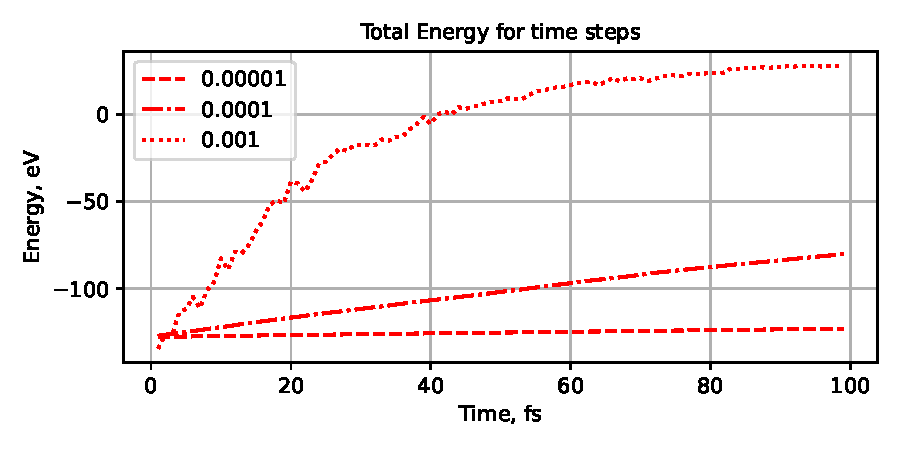
\includegraphics[width=.7\linewidth]{img/fig_total_energy.pdf}
	\caption{Total energy behaviour is better with very small time step.}
	\label{fig:first_simulation}
\end{figure*}


\subsection*{Berendsen thermostat}

\begin{figure*}[htb]
	\centering
	\begin{minipage}{.3\textwidth}
		\centering
		\resizebox{\columnwidth}{!}{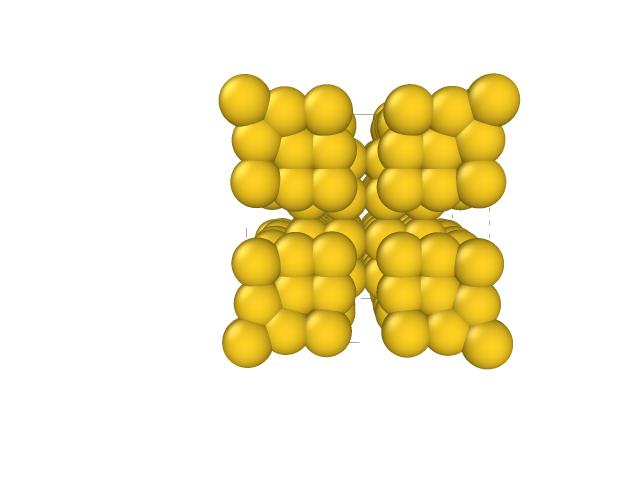
\includegraphics[trim={1.8cm 1.8cm 2.2cm 1.8cm},clip]{img/sim1.jpg}}
	\end{minipage}\hfill
	\begin{minipage}{.3\textwidth}
		\centering
		\resizebox{\columnwidth}{!}{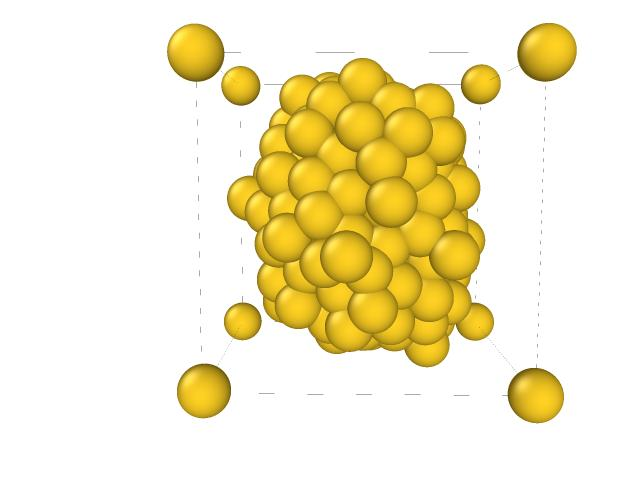
\includegraphics[trim={1.8cm 1.8cm 2.2cm 1cm},clip]{img/sim2.jpg}}
	\end{minipage}\hfill
	\begin{minipage}{.3\textwidth}
		\centering
		\resizebox{\columnwidth}{!}{
			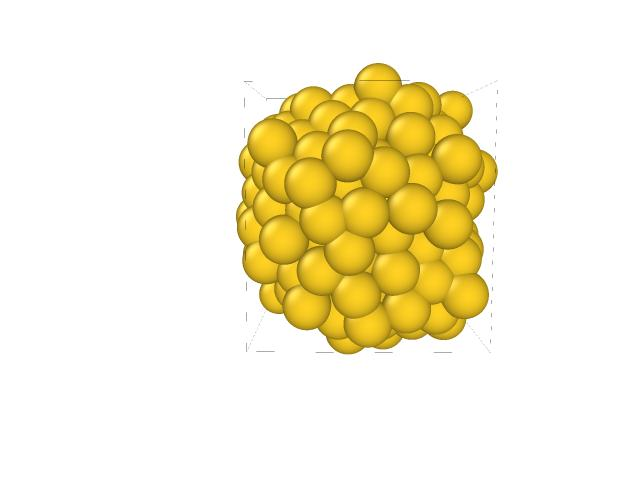
\includegraphics[trim={1.8cm 1.8cm 2.2cm 1cm},clip]{img/sim3.jpg}}
	\end{minipage}
	\caption{OVITO visualization of a cubic lattice with Berendsen thermostat. Without thermostat, atoms vaporize even with the smallest time step.}
	\label{fig:first_simulation_ovito}
\end{figure*}


I create a cube of atoms of width 4 for this experiment, Fig.~\ref{fig:first_simulation_ovito}

Choosing target temperature: 0.05 --- visualization shows that the atoms are pushed apart into infinity in small groups; 0.005 --- no vaporization.

Choosing Berendsen relaxation time: for the whole simulation, \(1000\Delta t\) is required to keep the atoms from evaporating; initial stronger relaxation doesn't make a difference.

Testing the Berendsen implementation is very simple, because it modifies the speed of each atom separately, so it's enough to test the behaviour on just one atom. I tested that the temperature should exponentially approach the wished value, and in case the relaxation time is equal to \(\Delta t\), it should change instantly.

{\bf Implementation} --- src/lattice.cpp, src/lattice.h, src/thermostat.cpp, src/thermostat.h, tests/test\_thermostat.cpp milestones/05/main.cpp

\subsection*{Neighbor list}

\begin{figure*}[htb]
	\centering
	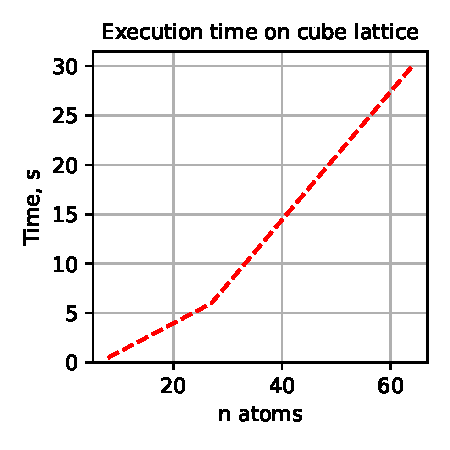
\includegraphics[width=.3\linewidth]{img/fig_pairwise.pdf}
	\caption{Time scales quadratically with number of atoms.}
	\label{fig:berendsen_time_pair}
\end{figure*}

\begin{figure*}[htb]
	\centering
	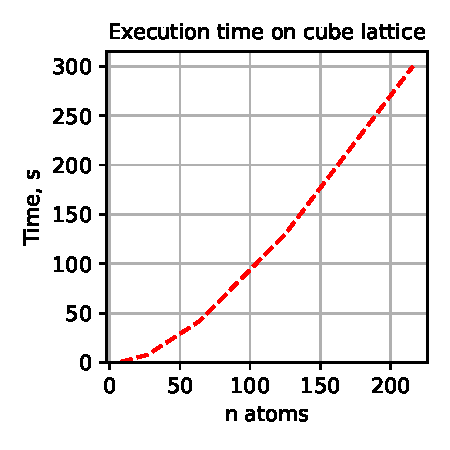
\includegraphics[width=.3\linewidth]{img/fig_neighbor.pdf}
	\caption{Time scales linearly with number of atoms.}
	\label{fig:berendsen_time_neighbor}
\end{figure*}

The provided implementation is used. Cutoff radius is \( 4 \sigma \) to allow speedup, but not miss important interactions. Execution time on clusters of different sizes is compared in Fig.~\ref{fig:berendsen_time_pair} and Fig.~\ref{fig:berendsen_time_neighbor}

{\bf Implementation} --- src/neighbors.cpp, src/neighbors.h, tests/test\_neighbors.cpp, src/lj.cpp, src/lj.h, tests/test\_thermostat.cpp milestones/05/main.cpp

\section{Conclusion}
\label{conclusion}

I should have planned to complete the project much earlier. The MPI part is well known, but it takes a lot of time to adapt the simulation code and debug.

\newpage
{\small
	\bibliographystyle{plain}
	\bibliography{egbib}
}

\end{document}
